\documentclass[12pt]{article}

\usepackage{graphicx}
\usepackage[left=0.8in,top=0.8in,right=0.8in,bottom=0.8in]{geometry}
\usepackage{titling}
\usepackage{sectsty}
\usepackage{comment}
\usepackage{amsmath}
\usepackage{amssymb}
\usepackage{siunitx}
\usepackage{float}
\graphicspath{{img/}}
\setlength\parindent{24pt}
\sectionfont{\fontsize{12}{16}\selectfont}

\title{\vspace{-2.5em} \Large \textbf{Homework \#3}}
\author{Justin Kang \\ AST 381: Planetary Astrophysics}
\date{\vspace{-0.75em} October 31, 2017}

\begin{document}
\maketitle

\section*{Introduction}
All code can be found under \texttt{src/}. The code was written in Python 3.6. \texttt{main.py} is the script that runs all parts of the assignment, \texttt{star.py} and \texttt{dust.py} are classes representing those two objects, and \texttt{util.py} is used for constants and useful utility functions. The \texttt{SHOW} array in \texttt{main.py} can be changed to adjust what output is displayed. All images can be found in \texttt{img/}.\\
\indent The star we are interested in for this project is Fomalhaut. Fomalhaut has a mass of 1.92 M$_{\odot}$, a radius of 1.842 R$_{\odot}$, a temperature of 8590 K, and is 7.70 pc away from us. For the dust, we are interested in "astrosilicate" of 0.1, 1, 10, and 1000 microns with different $Q_{abs}$. The $Q_{abs}$ and the corresponding wavelengths are found in \texttt{0.1micron.txt}, \texttt{1micron.txt}, and \texttt{10micron.txt} (we consider the 1000 micron dust as a perfect absorber, thus $\forall\lambda.\ Q_{abs} = 1$), with the original file from Princeton available in \texttt{dust.txt} \cite{dust}. All emission spectra are shown in units of microns and Jansky (Jy); in SI units, this is $10^{-26}$ \si{\watt\per\square\meter\per\hertz}.


\section{Spectra of Fomalhaut}
\begin{comment}
Write a computer code that takes stellar properties (temperature and radius) as input, and computes the flux density in Jansky (energy per unit time per unit area per unit frequency) at a user-specified orbital radius. That is, it should produce the properly flux-calibrated spectrum that would be seen by a spectrograph with 100% throughput and no slit losses. It’s fine to approximate the star as a blackbody. Test it for Fomalhaut, at orbital radii of 10 AU and 130 AU, and plot the resulting spectra.
\end{comment}
We first find the specific intensity through Planck's law, $B_{\nu}(\nu,T)$, using Fomalhaut's temperature and a specified frequency range (here $10^{13}-10^{15}$ Hz was used). We then integrate over the solid angle (in this case, multiply by $\pi$) to convert this to flux density. Finally we multiply this by the square of the ratio of the stellar and orbital radii to find the flux density at those orbital radii (assuming a circular orbit). The resulting spectra are shown in Figure 1.


\section{Power Absorbed by Dust}
\begin{comment}
Write a computer code that takes the output of Part 1, and calculates the total power absorbed by a dust grain of “astrosilicate” if it has a size of 0.1 microns, 1 micron, or 10 microns, or by a perfect absorber with a radius of 1 millimeter. Test it on each dust grain type at 10 AU and 130 AU away from Fomalhaut.
\end{comment}
We create all of the dust instances and read in the relevant $Q_{abs}$ and wavelengths from the files. Here the input frequencies used were just the ones corresponding to the given wavelengths. The absorbed power is given by the equation $$P_{in} = \pi r^{2}\int F_{in,\nu}Q_{abs}(\nu)d\nu.$$ Here $r$ is the radius of the dust and $\nu$ is obtained from the relation $\lambda\nu = c$. $F_{in}$ is the absorbed flux from the star, which is obtained from the corresponding orbital radius/value from part 1. The resulting absorbed powers are shown in Figure 2.


\section{Equilibrium Temperatures and Emission Spectra of Dust}
\begin{comment}
Write a computer code that takes the output of Part 2, and computes the equilibrium temperature and emission spectrum for a dust grain of each size/type. Be sure to appropriately account for the Q term in the emission spectrum as well. Again, test it on each dust grain type and at 10 AU and 130 AU away from Fomalhaut, calculating the temperature and luminosity and making a plot of the spectrum in each case.
\end{comment}
If the dust is a perfect absorber, we can treat it like a blackbody and use the equation $$P_{in} = P_{out} = 4\pi{r}^{2}\sigma{T}^{4}$$ to calculate the equilibrium temperature. If it is not a perfect absorber, then we must consider physical effects. Due to the difficulty for dust to emit light at wavelengths comparable to its size, we know that the dust will have a higher equilibrium temperature than if it was a blackbody. Using the equation $$P_{in} = P_{out} = 4\pi{r}^{2}\int\pi B_{\nu}(\nu,T)Q_{abs}(\nu)d\nu,$$ we binary search over $T$ to find the value that correctly matches the incoming and outgoing powers to find the equilibrium temperature for imperfect dust. The resulting equilibrium temperatures are shown in Figure 2.\\
\indent For perfect dust, we repeat the process we did in part 1 to produce the emission spectrum. For imperfect dust, we include the factor $Q_{abs}$ when integrating Planck's law over frequency. Here the orbital radius is taken to be the distance between us and Fomalhaut. The resulting spectra are shown in Figures 3 and 4. 


\section{Dust Count and Mass}
\begin{comment}
Go dig up an infrared+millimeter SED of Fomalhaut’s two (warm+cold) debris belts out of the literature, and compare it to the SEDs computed in Part 3. For each dust grain size/type, how many dust grains are needed to roughly match the observed SED of each component? What is the corresponding dust mass, if you assume the Fomalhaut debris ring is made out of grains of that size and that dust grains have a density somewhere around 2 g/cc? Which dust grain size produces the best fit to the SED shape?
\end{comment}
The reference SED for Fomalhaut's two debris belts was obtained from Su et al. (2013) \cite{sed}. Qualitatively, it appears that the flux densities of the warm and cold debris belts (with temperatures $\sim170$ and $\sim50$ K) have maximums of $10^{2.5}$ and $10^{4}$ Jy, respectively. We divide these maxima by those of the individual grains from part 2 to find roughly the number of dust grains we need to match the observed SED (we assume that each orbital radius has only one type of dust). Assuming that the dust grains have density 2 \si{\gram\per\cubic\centi\meter}, we multiply this by the volume $\frac{4}{3}\pi{r}^{3}$ (assuming the dust is spherical) and amount to find the total dust mass. Based on both qualitative appearance from part 3 and from matching temperatures from part 3 with Su et al, the dust grain sizes that produce the best fits to the SED shape are 1 mm at 10 AU and 10 \si{\micro} at 130 AU. The resulting number and masses are shown in Figure 5.


\section{Radiation Pressure and Poynting-Robertson Drag}
\begin{comment}
In class we talked about radiation pressure and Poynting-Robertson drag in terms of ideal blackbodies. However, for previous problems you’ve already calculated the actual energy absorption and emission of real particles, which should allow you to calculate better versions of each force. For each particle size, calculate the real radiation pressure and Poynting-Robertson drag at each radius. Estimate a characteristic timescale for dust grains of each size to be removed from the system, assuming they start at 10 AU or 130 AU.
\end{comment}
The force from radiation pressure is calculated using $F_{RP} = \frac{1}{c}P_{in}$. The force from Poynting-Robertson drag is calculated using $F_{PR} = \frac{v}{c^{2}}P_{in} = \frac{\sqrt{GM_{\star}/a}}{c^{2}}P_{in}$. Here $P_{in}$ is just the absorbed power from the star calculated in part 2. For characteristic timescales, we can get an approximation using the $\beta$ value, the square of the ratio of the forces from radiation pressure and gravity. If $\beta > 1$, we know that the force from radiation pressure is greater than the force of gravity and the dust will immediately be blown out of the system. Otherwise the timescale for Poynting-Robertson drag to remove the dust from the system is given by the equation \cite{timescale} $$\tau = \frac{1}{4}\left(\frac{GM_{\star}\beta}{c}\right)^{-1}\left(a^{2}-R_{\star}^{2}\right).$$ The forces and the removal scales are shown in Figure 6.


\bibliographystyle{ieeetr}
\bibliography{mybib}

\section*{Appendix}
\vspace{-1em}
% Fomalhaut's spectra from 10 and 130 AU
\begin{figure}[H]
\centering
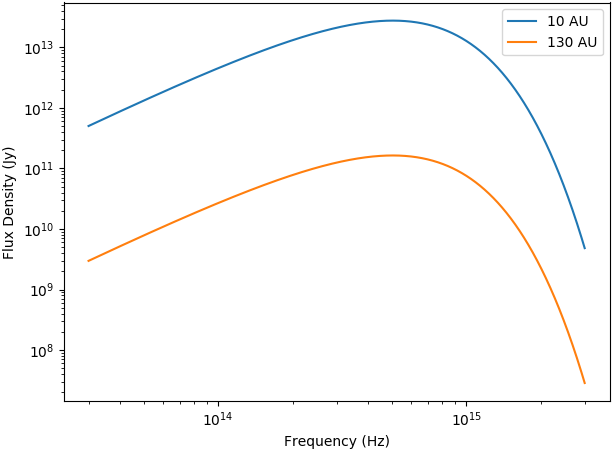
\includegraphics[width=0.75\textwidth]{star.png}
\vspace{-0.5em}
\caption{The SED of Fomalhaut.}
\end{figure}

% The dust's absorbed powers and equilibrium temperatures
\begin{figure}[H]
\centering
\begin{tabular}{ |c|c|c|c| } 
\hline
r (\si{\micro}) & a (AU) & Absorbed Power (W) & Equilibrium Temp (K)\\
\hline
0.1 & 10 & $1.466*10^{-12}$ & 259.8\\
1 & 10 & $6.251*10^{-10}$ & 212.6\\
10 & 10 & $6.599*10^{-8}$ & 159.1\\
1000 & 10 & $7.117*10^{-4}$ & 177.8\\

0.1 & 130 & $8.674*10^{-15}$ & 97.8\\
1 & 130 & $3.699*10^{-12}$ & 83.4\\
10 & 130 & $3.905*10^{-10}$ & 48.5\\
1000 & 130 & $4.211*10^{-6}$ & 49.3\\
\hline
\end{tabular}
\caption{The absorbed power and equilibrium temperatures of the different dust.}
\end{figure}

% The dust's spectra from 7.7 pc
\begin{figure}[H]
\centering
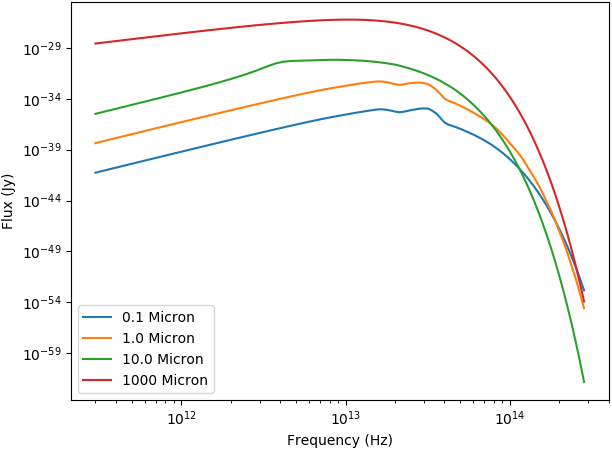
\includegraphics[width=0.75\textwidth]{near_dust.png}
\vspace{-0.5em}
\caption{The SEDs of the individual dust grains at 10 AU}
\end{figure}

% The dust's spectra from 7.7 pc
\begin{figure}[H]
\centering
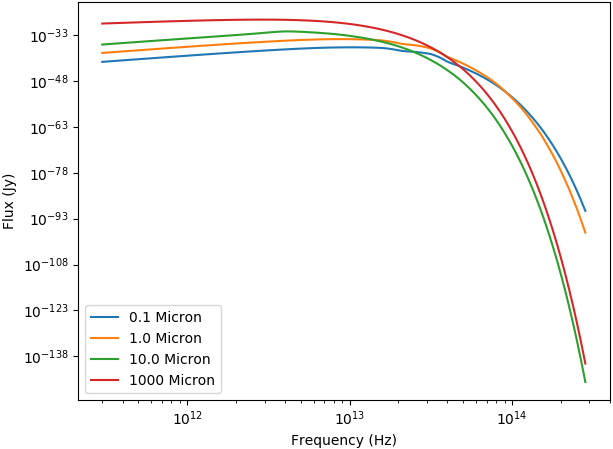
\includegraphics[width=0.75\textwidth]{far_dust.png}
\vspace{-0.5em}
\caption{The SEDs of the individual dust grains at 130 AU.}
\end{figure}

% The number and masses of the dust
\begin{figure}[H]
\centering
\begin{tabular}{ |c|c|c|c| } 
\hline
r (\si{\micro}) & a (AU) & Number of Dust Grains & Total Mass (kg)\\
\hline
0.1 & 10 & $2.807*10^{34}$ & $2.352*10^{17}$\\
1 & 10 & $6.241*10^{31}$ & $5.229*10^{17}$\\
10 & 10 & $4.702*10^{29}$ & $3.939*10^{18}$\\
1000 & 10 & $5.336*10^{25}$ & $4.470*10^{20}$\\

0.1 & 130 & $9.062*10^{37}$ & $7.592*10^{20}$\\
1 & 130 & $1.899*10^{35}$ & $1.591*10^{21}$\\
10 & 130 & $5.693*10^{32}$ & $4.770*10^{21}$\\
1000 & 130 & $7.912*10^{28}$ & $6.628*10^{23}$\\
\hline
\end{tabular}
\caption{The number of dust grains and subsequent mass needed to match the reference SED.}
\end{figure}

% The RP, PR drag, and removal timescales of the dust
\begin{figure}[H]
\centering
\begin{tabular}{ |c|c|c|c|c| } 
\hline
r (\si{\micro}) & a (AU) & Radiation Pressure (N) & P-R Drag (N) & Removal Time (yr)\\
\hline
0.1 & 10 & $4.890*10^{-21}$ & $2.219*10^{-25}$ & $0$\\
1 & 10 & $2.085*10^{-18}$ & $9.077*10^{-23}$ & $0$\\
10 & 10 & $2.201*10^{-16}$ & $9.582*10^{-21}$ & $9.045*10^{4}$\\
1000 & 10 & $2.374*10^{-12}$ & $1.033*10^{-16}$ & $8.387*10^{6}$\\

0.1 & 130 & $2.893*10^{-23}$ & $3.494*10^{-28}$ & $0$\\
1 & 130 & $1.234*10^{-20}$ & $1.490*10^{-25}$ & $0$\\
10 & 130 & $1.302*10^{-18}$ & $1.573*10^{-23}$ & $1.529*10^{7}$\\
1000 & 130 & $1.405*10^{-14}$ & $1.696*10^{-19}$ & $1.417*10^{9}$\\
\hline
\end{tabular}
\caption{The absorbed power and equilibrium temperatures of the different dust.}
\end{figure}


\end{document}